\documentclass[letterpaper,11pt]{article}

\oddsidemargin 0.0in
\evensidemargin 0.0in
\textwidth 6.5in
%\headheight 0.0in

\usepackage{graphics}
\usepackage{amsmath}
\usepackage{indentfirst}
\usepackage{tabularx}
\usepackage{graphicx}
\usepackage{url}
\usepackage{appendix}
\usepackage{verbatim}
\usepackage{lscape}
\usepackage{rotating}
\usepackage{longtable}



\DeclareMathOperator{\var}{var}
\DeclareMathOperator{\cov}{cov}

\usepackage{Sweave}
\begin{document}

\title{\texttt{multilevelPSA}: An R Package for Multilevel Propensity Score Analysis}
\author{Jason M. Bryer\\
\small{}jbryer@bryer.org}
\date{\today}

\maketitle

\abstract{The use of propensity score analysis (Rosenbaum \& Rubin, 1983) has gained increasing popularity for the estimation of causal effects within observational studies. However, its use in situations where data is multilevel, or clustered, is limited (Arpino \& Mealli, 2008). This talk will introduce the multilevelPSA (Bryer, 2011) package for R that provides functions for estimating propensity scores for large datasets using logistic regression and conditional inference trees. Furthermore, a set of graphical functions that extends the framework of visualizing propensity score analysis introduced by Helmreich and Pruzek (2009) to multilevel analysis will be discussed. An application for estimating the effects of private schools on reading, mathematics, and science outcomes from the Programme for International Student Assessment (PISA; Organization for Economic Co-operation and Development, 2009) is provided.
\ \\ \ \\
\noindent Keywords: \textit{PSA, propensity score analysis, multilevel, graphics}}



\section{Introduction}

The \texttt{multilevelPSA} package is hosted on github. The latest developmental version can be installed using the \texttt{devtools} package.

\begin{Schunk}
\begin{Sinput}
> library(devtools)
> install_github('multilevelPSA', 'jbryer')
\end{Sinput}
\end{Schunk}

Now we can load and list the available functions.

\begin{Schunk}
\begin{Sinput}
> library(multilevelPSA)
> ls('package:multilevelPSA')
\end{Sinput}
\begin{Soutput}
 [1] "GeomRugAlt"                   "geom_rug_alt"                
 [3] "getPropensityScores"          "getStrata"                   
 [5] "missingPlot"                  "multilevelCtree"             
 [7] "multilevelLR"                 "multilevelPSA"               
 [9] "plot.multilevel.distribution" "plotcirc.multilevel.psa"     
[11] "plotpsa.multilevel.psa"       "treeHeat"                    
\end{Soutput}
\end{Schunk}


\section{Programme for International Student Achievement}

\url{http://www.pisa.oecd.org/}

\begin{Schunk}
\begin{Sinput}
> data(pisa.student)
> nrow(student.orig)
\end{Sinput}
\begin{Soutput}
[1] 475460
\end{Soutput}
\begin{Sinput}
> data(pisa.school)
> nrow(school.orig)
\end{Sinput}
\begin{Soutput}
[1] 17145
\end{Soutput}
\end{Schunk}


\begin{Schunk}
\begin{Sinput}
> school = school.orig[,c('COUNTRY', "CNT", "SCHOOLID",
+ 	"SC02Q01", #Public (1) or private (2)
+ 	"STRATIO" #Student-teacher ration    
+ )]
> names(school) = c('COUNTRY', 'CNT', 'SCHOOLID', 'PUBPRIV', 'STRATIO')
> school$SCHOOLID = as.integer(school$SCHOOLID)
> rm(school.orig)
\end{Sinput}
\end{Schunk}

% latex table generated in R 2.14.0 by xtable 1.6-0 package
% Mon Nov 14 10:55:14 2011
\begin{longtable}{rrr}
\caption{Number of Private and Public Schools by Country} \\ 
  \hline
  Public & Private & Missing \\ \endfirsthead \multicolumn{3}{l}{{...continued from previous page}}\\ \hline Public & Private & Missing  \\ \hline \endhead \hline
164 &  17 &   0 \\ 
  158 &   4 &   0 \\ 
  141 &  58 &   0 \\ 
  217 & 136 &   0 \\ 
  234 &  39 &   9 \\ 
   89 & 189 &   0 \\ 
  812 &  98 &  37 \\ 
  174 &   4 &   0 \\ 
  896 &  76 &   6 \\ 
   80 & 103 &  17 \\ 
  137 &  15 &   0 \\ 
   97 &  61 &   0 \\ 
  222 &  51 &   2 \\ 
  154 &   4 &   0 \\ 
  234 &  15 &  12 \\ 
  231 &  50 &   4 \\ 
  168 &   7 &   0 \\ 
  191 &  12 &   0 \\ 
    0 &   0 & 168 \\ 
  202 &  11 &  13 \\ 
  173 &  11 &   0 \\ 
   10 & 140 &   1 \\ 
  163 &  24 &   0 \\ 
  112 &   2 &  17 \\ 
   85 &  98 &   0 \\ 
   57 &  87 &   0 \\ 
  140 &  31 &   5 \\ 
  987 &  84 &  26 \\ 
  135 &  51 &   0 \\ 
  191 &   8 &   0 \\ 
  181 &  29 &   0 \\ 
   99 &  58 &   0 \\ 
  167 &   6 &   0 \\ 
  181 &   3 &   0 \\ 
   10 &   2 &   0 \\ 
  193 &   2 &   1 \\ 
   30 &   9 &   0 \\ 
    3 &  42 &   0 \\ 
  1332 & 200 &   3 \\ 
   50 &   2 &   0 \\ 
   69 & 113 &   4 \\ 
  153 &  10 &   0 \\ 
  186 &   4 &   7 \\ 
  136 &  40 &  12 \\ 
  189 &  51 &   0 \\ 
  166 &  19 &   0 \\ 
  185 &  29 &   0 \\ 
   88 &  59 &   6 \\ 
  158 &   1 &   0 \\ 
  212 &   1 &   0 \\ 
  184 &   3 &   3 \\ 
  167 &   4 &   0 \\ 
  172 &  17 &   0 \\ 
  336 &   5 &   0 \\ 
  512 & 359 &  18 \\ 
  159 &  30 &   0 \\ 
  399 &  22 &   5 \\ 
  204 &  26 &   0 \\ 
  120 &  32 &   6 \\ 
   44 & 146 &   0 \\ 
  148 &  17 &   0 \\ 
  169 &   1 &   0 \\ 
  439 &  17 &  26 \\ 
  154 &  11 &   0 \\ 
  193 &  39 &   0 \\ 
   \hline
\hline
\label{ppxtab}
\end{longtable}
% latex table generated in R 2.14.0 by xtable 1.6-0 package
% Mon Nov 14 10:55:14 2011
\begin{longtable}{lll}
\caption{Covariates Used for Propensity Score Estimations} \\ 
  \hline
  Variable & Name & Description \\ \endfirsthead \multicolumn{3}{l}{{...continued from previous page}}\\ \hline Variable & Name & Description  \\ \hline \endhead \hline
CNT & CNT & Country \\ 
  SCHOOLID & SchoolId & SchoolID \\ 
  StIDStd & StudentId & Student ID \\ 
  ST01Q01 & Grade & Grade \\ 
  ST04Q01 & Sex & Sex \\ 
  ST05Q01 & Attend & Attend \\ 
  ST06Q01 & Age & Age \\ 
  ST07Q01 & Repeat & Repeat \\ 
  ST08Q01 & Mother & At home mother \\ 
  ST08Q02 & Father & At home father \\ 
  ST08Q03 & Brother & At home brothers \\ 
  ST08Q04 & Sister & At home sisters \\ 
  ST08Q05 & GrandPa & At home grandparents \\ 
  ST08Q06 & Other & At home others \\ 
  ST10Q01 & MomEd & Mother highest schooling \\ 
  ST12Q01 & MomJob & Mother current job status \\ 
  ST14Q01 & DadEd & Father highest schooling \\ 
  ST16Q01 & DadJob & Father current job status \\ 
  ST19Q01 & Lang & Language at home \\ 
  ST20Q01 & Desk & Desk \\ 
  ST20Q02 & OwnRoom & Own room \\ 
  ST20Q03 & StudyPl & Study place \\ 
  ST20Q04 & Computer & Computer \\ 
  ST20Q05 & Software & Software \\ 
  ST20Q06 & Internet & Internet \\ 
  ST20Q07 & Lit & Literature \\ 
  ST20Q08 & Poetry & Poetry \\ 
  ST20Q09 & Art & Art \\ 
  ST20Q10 & TxtBooks & Textbooks \\ 
  ST20Q12 & Dict & Dictionary \\ 
  ST20Q13 & DishW & Dishwasher \\ 
  ST20Q14 & DVD & DVD \\ 
  ST21Q01 & CellPh & How many cellphones \\ 
  ST21Q02 & TVs & How many TVs \\ 
  ST21Q03 & nComp & How many computers \\ 
  ST21Q04 & nCars & How many cars \\ 
  ST21Q05 & nBaths & How many rooms bath or shower \\ 
  ST22Q01 & nBooks & How many books \\ 
  ST23Q01 & Reading & Reading enjoyment time \\ 
  ST31Q01 & EnrichLang & Enrich in test language \\ 
  ST31Q02 & EnrichMath & Enrich in mathematics \\ 
  ST31Q03 & EnrichScie & Enrich in science \\ 
  ST31Q05 & RemedialLang & Remedial in test language \\ 
  ST31Q06 & RemedialMath & Remedial in mathematics \\ 
  ST31Q07 & RemedialScie & Remedial in science \\ 
  ST32Q01 & LangLessons & Out of school lessons in test language \\ 
  ST32Q02 & MathLessons & Out of school lessons maths \\ 
  ST32Q03 & ScieLessons & Out of school lessons in science \\ 
   \hline
\hline
\label{covariates}
\end{longtable}
We will only use countries with at least 10 private schools.

\begin{Schunk}
\begin{Sinput}
> t = as.data.frame(table(school$CNT, school$PUBPRIV))
> t = cast(t, Var1 ~ Var2, value='Freq')
> countries = t[which(t$Private >= 10), 'Var1']
> student = student.orig[which(student.orig$CNT %in% countries), psa.cols]
> rm(student.orig)
\end{Sinput}
\end{Schunk}

The \texttt{recodePISA} function will convert the columns to factor variables.

\begin{Schunk}
\begin{Sinput}
> student$CNT = as.character(student$CNT)
> student = ddply(student, 'CNT', recodePISA, .progress='text')
\end{Sinput}
\end{Schunk}

Merge the school data with the student data.

\begin{Schunk}
\begin{Sinput}
> student = merge(student, school, by=c('CNT', 'SCHOOLID'), all.x=TRUE)
> student = student[!is.na(student$PUBPRIV),] #Remove rows with missing PUBPRRIV
\end{Sinput}
\end{Schunk}

\section{Missingness}

Figure \ref{fig:missing plot} represents the extent of missingness across the covariates and variables. The \texttt{mice} package is used to impute missing values.

\begin{figure}[tp]
\begin{center}
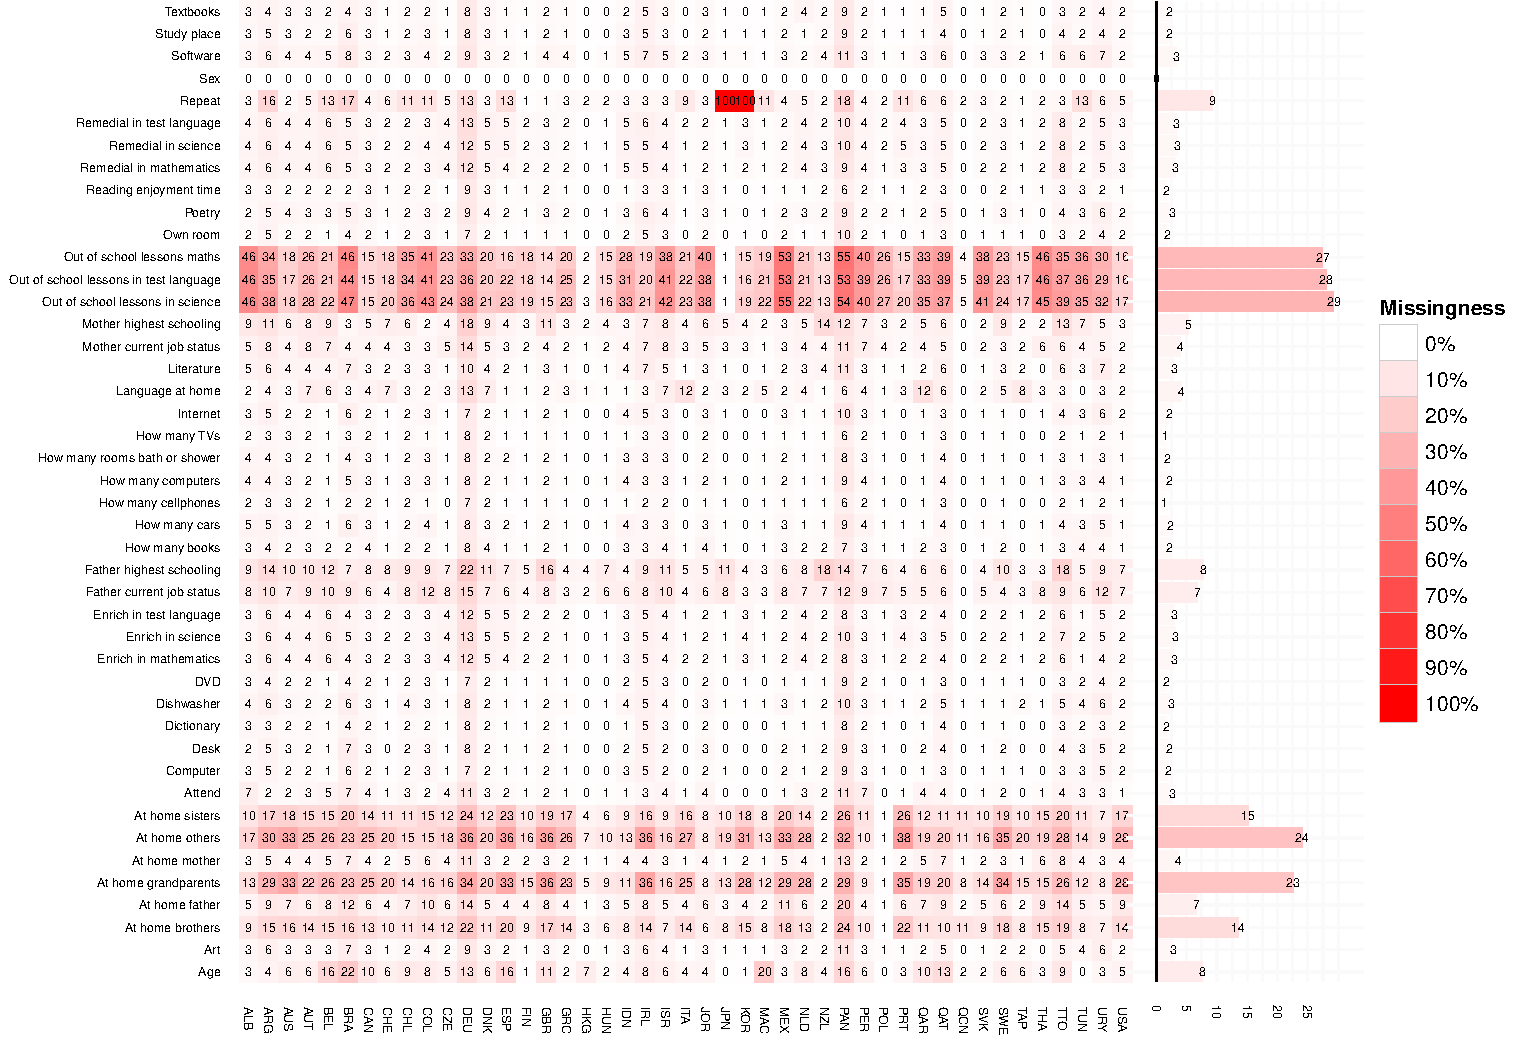
\includegraphics[width=\textwidth]{figures/MissingPlot.pdf}
\caption{Missing Data Plot}
\label{fig:missingplot}
\end{center}
\end{figure}


\section{Conditional Inference Trees}


\begin{Schunk}
\begin{Sinput}
> party.results = multilevelCtree(student[,c(1,5:48,68)], formula=PUBPRIV ~ ., level2='CNT')
\end{Sinput}
\end{Schunk}


\begin{Schunk}
\begin{Sinput}
> party.results[['USA']]
\end{Sinput}
\begin{Soutput}
	 Conditional inference tree with 9 terminal nodes

Response:  PUBPRIV 
Inputs:  ST04Q01, ST05Q01, ST06Q01, ST07Q01, ST08Q01, ST08Q02, ST08Q03, ST08Q04, ST08Q05, ST08Q06, ST10Q01, ST12Q01, ST14Q01, ST16Q01, ST19Q01, ST20Q01, ST20Q02, ST20Q03, ST20Q04, ST20Q05, ST20Q06, ST20Q07, ST20Q08, ST20Q09, ST20Q10, ST20Q12, ST20Q13, ST20Q14, ST21Q01, ST21Q02, ST21Q03, ST21Q04, ST21Q05, ST22Q01, ST23Q01, ST31Q01, ST31Q02, ST31Q03, ST31Q05, ST31Q06, ST31Q07, ST32Q01, ST32Q02, ST32Q03 
Number of observations:  5233 

1) ST22Q01 <= 4; criterion = 1, statistic = 156.494
  2) ST20Q07 == {Yes}; criterion = 1, statistic = 54.294
    3) ST21Q03 <= 3; criterion = 0.984, statistic = 12.669
      4)*  weights = 772 
    3) ST21Q03 > 3
      5)*  weights = 414 
  2) ST20Q07 == {No}
    6) ST21Q05 <= 3; criterion = 1, statistic = 24.064
      7) ST21Q03 <= 2; criterion = 0.998, statistic = 16.223
        8)*  weights = 1391 
      7) ST21Q03 > 2
        9)*  weights = 1261 
    6) ST21Q05 > 3
      10)*  weights = 501 
1) ST22Q01 > 4
  11) ST21Q05 <= 3; criterion = 1, statistic = 21.974
    12) ST04Q01 == {Male}; criterion = 0.993, statistic = 14.227
      13)*  weights = 245 
    12) ST04Q01 == {Female}
      14) ST31Q06 == {Yes}; criterion = 0.986, statistic = 12.995
        15)*  weights = 19 
      14) ST31Q06 == {No}
        16)*  weights = 275 
  11) ST21Q05 > 3
    17)*  weights = 355 
\end{Soutput}
\end{Schunk}

\begin{figure}[tp]
\begin{center}
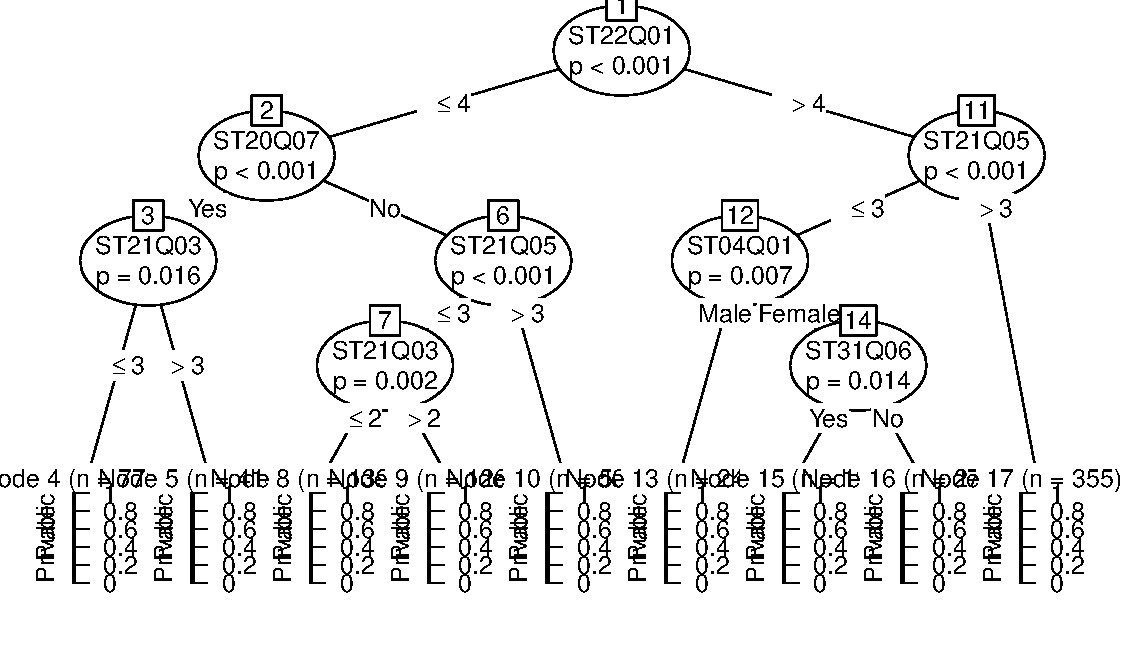
\includegraphics{multilevelPSA-014}
\caption{Classification Tree for USA}
\label{fig:usatree}
\end{center}
\end{figure}

The \texttt{getStrata} function add a variable to the \texttt{student} data frame indicating the leaf node each record belongs to. This is analogous to using the fitted values from logistic regression models except for classification trees the resulted ``fitted" values are categorical.

\begin{Schunk}
\begin{Sinput}
> student.party = getStrata(party.results, student, level2='CNT')
> student.party$mathscore = apply(student.party[,c('PV1MATH','PV2MATH','PV3MATH','PV4MATH','PV5MATH')], 1, sum) / 5
> student.party$readscore = apply(student.party[,c('PV1READ','PV2READ','PV3READ','PV4READ','PV5READ')], 1, sum) / 5
> student.party$sciescore = apply(student.party[,c('PV1SCIE','PV2SCIE','PV3SCIE','PV4SCIE','PV5SCIE')], 1, sum) / 5
\end{Sinput}
\end{Schunk}



\begin{figure}[tp]
\begin{center}
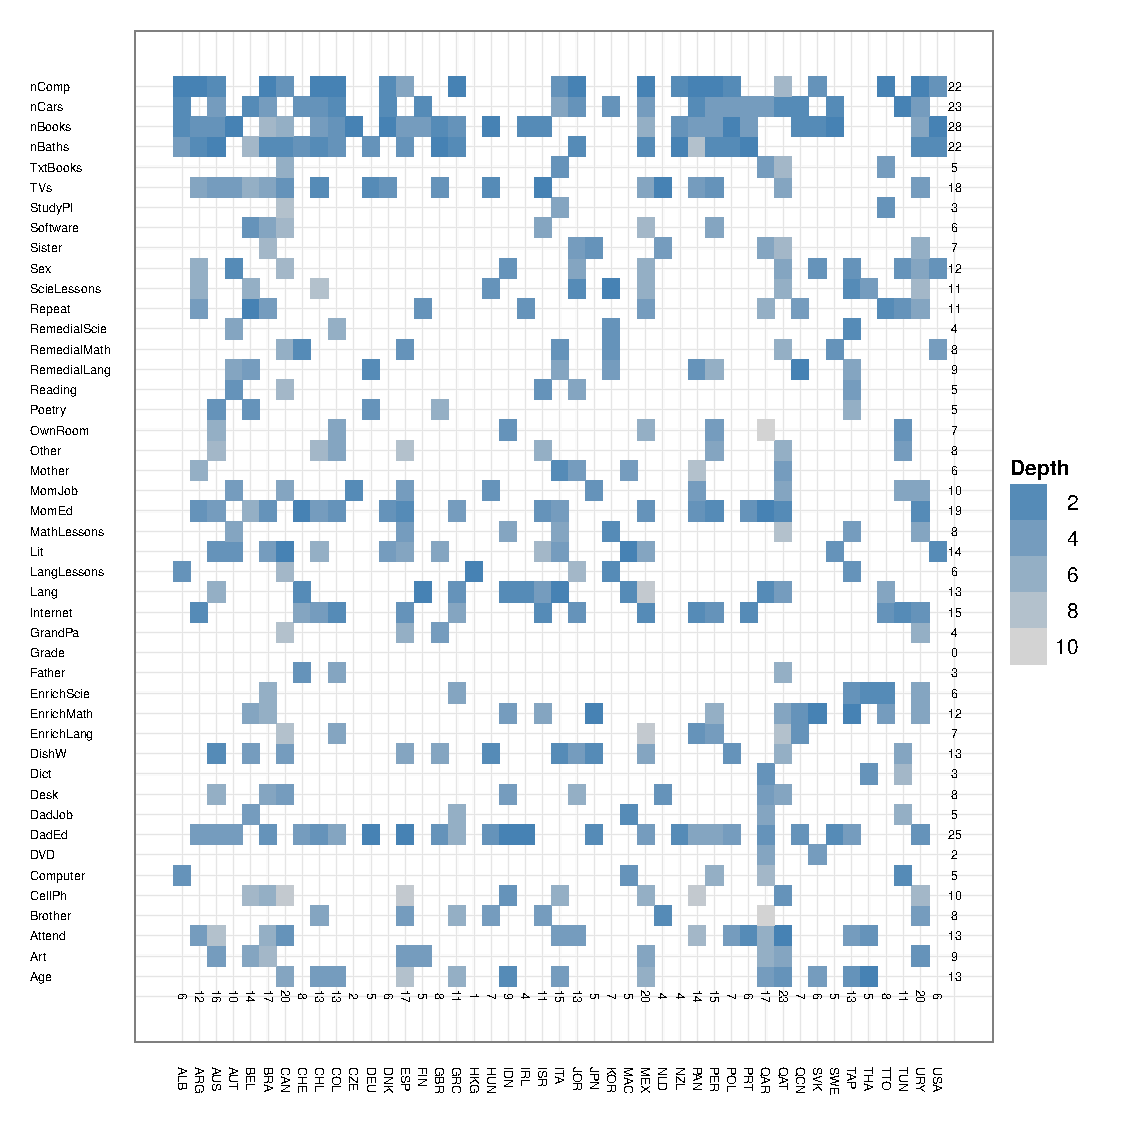
\includegraphics{multilevelPSA-017}
\caption{Heat Map of Relative Importance of Covariates for Classification Tree}
\label{fig:treeheat}
\end{center}
\end{figure}

\section{Multilevel Propensity Score Analysis}

The \texttt{multilevlePSA} function will estimate the model. It returns a list of objects.

\begin{Schunk}
\begin{Sinput}
> results.psa.math = multilevelPSA(response=student.party$mathscore,
+ treatment=student.party$PUBPRIV, strata=student.party$strata, level2=student.party$level2, minN=5)
> results.psa.math$level2.summary
\end{Sinput}
\begin{Soutput}
   level2     n     diffwtd      mnx      mny     mnxy     ci.min     ci.max
1     ALB  4596  47.3790192 373.4865 420.8655 397.1760  37.112435  57.645604
2     ARG  4707  28.2484795 381.7359 409.9844 395.8602  19.860348  36.636611
3     AUS 14251  28.1066901 497.6153 525.7220 511.6686  23.477031  32.736349
4     AUT  6405  -6.1648792 500.5522 494.3873 497.4697 -16.364671   4.034913
5     BEL  8488  40.1158641 490.3529 530.4688 510.4108  32.093483  48.138245
6     BRA 19112  49.7071212 370.9140 420.6211 395.7676  44.353349  55.060893
7     CAN 23035  62.5228111 512.7358 575.2587 543.9973  54.954257  70.091366
8     CHE 11645   9.7261224 529.4889 539.2150 534.3519  -3.673243  23.125488
9     CHL  5122  17.8894194 414.0480 431.9374 422.9927   9.495447  26.283392
10    COL  7695  28.2621517 381.9667 410.2289 396.0978  22.435477  34.088827
11    CZE  5751   2.8407124 510.6293 513.4700 512.0497  -8.075300  13.756725
12    DEU  4555  19.2101332 510.5953 529.8054 520.2003   3.206619  35.213647
13    DNK  5839  14.3020577 486.4226 500.7247 493.5737   5.809685  22.794430
14    ESP 25363  17.0291397 484.6639 501.6931 493.1785  13.582441  20.475839
15    FIN  5755  -5.0068378 539.0456 534.0387 536.5422 -18.863984   8.850308
16    GBR  8202  37.2784671 501.2581 538.5366 519.8973  27.933956  46.622978
17    GRC  4665  21.7905098 468.1922 489.9827 479.0875  10.808237  32.772783
18    HKG  4804 -38.5730792 591.3133 552.7403 572.0268 -50.860842 -26.285316
19    HUN  4583   7.7575339 494.1992 501.9567 498.0780  -4.266093  19.781161
20    IDN  5136 -19.9146604 382.3154 362.4007 372.3581 -26.426146 -13.403175
21    IRL  3928  14.8558437 478.9441 493.7999 486.3720   3.175379  26.536309
22    ISR  5607  26.0632963 445.0270 471.0903 458.0587  15.921608  36.204985
23    ITA 30234 -27.3416112 491.9211 464.5795 478.2503 -37.826591 -16.856631
24    JOR  6439  30.2889397 389.4549 419.7438 404.5994  20.712494  39.865385
25    JPN  6088 -10.8692711 532.6987 521.8295 527.2641 -20.465999  -1.272544
26    KOR  4989   0.8395903 548.4127 549.2523 548.8325  -7.121606   8.800787
27    MAC  5628  46.9146659 480.8967 527.8113 504.3540  34.677379  59.151953
28    MEX 38124   7.4136629 422.9836 430.3973 426.6905   3.784570  11.042756
29    NLD  4667  -3.9098201 535.8870 531.9771 533.9321 -18.107778  10.288137
30    NZL  4643  53.9164073 519.8993 573.8157 546.8575  44.564926  63.267889
31    PAN  3608  65.3574564 344.0597 409.4171 376.7384  56.961259  73.753654
32    PER  5985  29.6893404 357.5425 387.2319 372.3872  19.766241  39.612440
33    POL  4803  25.9568444 496.4239 522.3807 509.4023  14.719257  37.194432
34    PRT  6298  19.6082394 483.6007 503.2090 493.4048  11.927275  27.289204
35    QAR  5287  67.6177694 386.7242 454.3420 420.5331  58.474855  76.760683
36    QAT  8277  65.5211793 344.5661 410.0873 377.3267  58.265664  72.776695
37    QCN  4966  30.3213774 597.5703 627.8917 612.7310  15.221133  45.421622
38    SVK  4555  22.0127982 494.3370 516.3498 505.3434   6.597103  37.428493
39    SWE  4567  24.2053941 492.3527 516.5581 504.4554  14.103703  34.307085
40    TAP  5831 -47.3761828 565.5145 518.1383 541.8264 -53.934452 -40.817914
41    THA  6209 -22.3318702 429.6974 407.3655 418.5314 -31.787698 -12.876042
42    TTO  4604 -11.6999857 419.4573 407.7573 413.6073 -19.900966  -3.499005
43    TUN  2414 -75.8419263 377.2423 301.4003 339.3213 -88.562235 -63.121618
44    URY  5462  52.7456587 416.3180 469.0636 442.6908  44.245235  61.246083
45    USA  5233  19.7061018 484.7964 504.5025 494.6495   7.267340  32.144863
      df   se.wtd    xmark    ymark
1   4578 5.236765 284.0948 331.4738
2   4681 4.278631 293.6601 321.9085
3  14193 2.361913 293.7310 321.8376
4   6377 5.203083 310.8667 304.7019
5   8460 4.092541 287.7264 327.8422
6  19032 2.731393 282.9307 332.6379
7  22979 3.861375 276.5229 339.0457
8  11625 6.835825 302.9212 312.6474
9   5098 4.281701 298.8396 316.7290
10  7651 2.972378 293.6532 321.9154
11  5745 5.568323 306.3639 309.2047
12  4545 8.163034 298.1792 317.3894
13  5825 4.332022 300.6333 314.9353
14 25295 1.758468 299.2697 316.2989
15  5741 7.068612 310.2877 305.2809
16  8176 4.766989 289.1451 326.4235
17  4643 5.601843 296.8890 318.6796
18  4800 6.267801 327.0708 288.4978
19  4569 6.132991 303.9055 311.6631
20  5116 3.321462 317.7416 297.8270
21  3916 5.957688 300.3564 315.2122
22  5585 5.173304 294.7527 320.8159
23 30208 5.349364 321.4551 294.1135
24  6411 4.885109 292.6398 322.9288
25  6070 4.895403 313.2189 302.3497
26  4961 4.060919 307.3645 308.2041
27  5618 6.242283 284.3270 331.2416
28 38036 1.851553 304.0775 311.4911
29  4657 7.242106 309.7392 305.8294
30  4631 4.770005 280.8261 334.7425
31  3568 4.282400 275.1056 340.4630
32  5941 5.061868 292.9396 322.6290
33  4787 5.732119 294.8059 320.7627
34  6286 3.918177 297.9802 317.5884
35  5225 4.663757 273.9754 341.5932
36  8163 3.701313 275.0237 340.5449
37  4954 7.702465 292.6236 322.9450
38  4547 7.863201 296.7779 318.7907
39  4555 5.152649 295.6816 319.8870
40  5805 3.345419 331.4724 284.0962
41  6191 4.823548 318.9502 296.6184
42  4592 4.183148 313.6343 301.9343
43  2404 6.486805 345.7053 269.8633
44  5414 4.336061 281.4115 334.1571
45  5215 6.344951 297.9313 317.6374
\end{Soutput}
\end{Schunk}

\begin{Schunk}
\begin{Sinput}
> options(digits=2)
> results.psa.math$level2.summary
\end{Sinput}
\begin{Soutput}
   level2     n diffwtd mnx mny mnxy ci.min ci.max    df se.wtd xmark ymark
1     ALB  4596   47.38 373 421  397   37.1   57.6  4578    5.2   284   331
2     ARG  4707   28.25 382 410  396   19.9   36.6  4681    4.3   294   322
3     AUS 14251   28.11 498 526  512   23.5   32.7 14193    2.4   294   322
4     AUT  6405   -6.16 501 494  497  -16.4    4.0  6377    5.2   311   305
5     BEL  8488   40.12 490 530  510   32.1   48.1  8460    4.1   288   328
6     BRA 19112   49.71 371 421  396   44.4   55.1 19032    2.7   283   333
7     CAN 23035   62.52 513 575  544   55.0   70.1 22979    3.9   277   339
8     CHE 11645    9.73 529 539  534   -3.7   23.1 11625    6.8   303   313
9     CHL  5122   17.89 414 432  423    9.5   26.3  5098    4.3   299   317
10    COL  7695   28.26 382 410  396   22.4   34.1  7651    3.0   294   322
11    CZE  5751    2.84 511 513  512   -8.1   13.8  5745    5.6   306   309
12    DEU  4555   19.21 511 530  520    3.2   35.2  4545    8.2   298   317
13    DNK  5839   14.30 486 501  494    5.8   22.8  5825    4.3   301   315
14    ESP 25363   17.03 485 502  493   13.6   20.5 25295    1.8   299   316
15    FIN  5755   -5.01 539 534  537  -18.9    8.9  5741    7.1   310   305
16    GBR  8202   37.28 501 539  520   27.9   46.6  8176    4.8   289   326
17    GRC  4665   21.79 468 490  479   10.8   32.8  4643    5.6   297   319
18    HKG  4804  -38.57 591 553  572  -50.9  -26.3  4800    6.3   327   288
19    HUN  4583    7.76 494 502  498   -4.3   19.8  4569    6.1   304   312
20    IDN  5136  -19.91 382 362  372  -26.4  -13.4  5116    3.3   318   298
21    IRL  3928   14.86 479 494  486    3.2   26.5  3916    6.0   300   315
22    ISR  5607   26.06 445 471  458   15.9   36.2  5585    5.2   295   321
23    ITA 30234  -27.34 492 465  478  -37.8  -16.9 30208    5.3   321   294
24    JOR  6439   30.29 389 420  405   20.7   39.9  6411    4.9   293   323
25    JPN  6088  -10.87 533 522  527  -20.5   -1.3  6070    4.9   313   302
26    KOR  4989    0.84 548 549  549   -7.1    8.8  4961    4.1   307   308
27    MAC  5628   46.91 481 528  504   34.7   59.2  5618    6.2   284   331
28    MEX 38124    7.41 423 430  427    3.8   11.0 38036    1.9   304   311
29    NLD  4667   -3.91 536 532  534  -18.1   10.3  4657    7.2   310   306
30    NZL  4643   53.92 520 574  547   44.6   63.3  4631    4.8   281   335
31    PAN  3608   65.36 344 409  377   57.0   73.8  3568    4.3   275   340
32    PER  5985   29.69 358 387  372   19.8   39.6  5941    5.1   293   323
33    POL  4803   25.96 496 522  509   14.7   37.2  4787    5.7   295   321
34    PRT  6298   19.61 484 503  493   11.9   27.3  6286    3.9   298   318
35    QAR  5287   67.62 387 454  421   58.5   76.8  5225    4.7   274   342
36    QAT  8277   65.52 345 410  377   58.3   72.8  8163    3.7   275   341
37    QCN  4966   30.32 598 628  613   15.2   45.4  4954    7.7   293   323
38    SVK  4555   22.01 494 516  505    6.6   37.4  4547    7.9   297   319
39    SWE  4567   24.21 492 517  504   14.1   34.3  4555    5.2   296   320
40    TAP  5831  -47.38 566 518  542  -53.9  -40.8  5805    3.3   331   284
41    THA  6209  -22.33 430 407  419  -31.8  -12.9  6191    4.8   319   297
42    TTO  4604  -11.70 419 408  414  -19.9   -3.5  4592    4.2   314   302
43    TUN  2414  -75.84 377 301  339  -88.6  -63.1  2404    6.5   346   270
44    URY  5462   52.75 416 469  443   44.2   61.2  5414    4.3   281   334
45    USA  5233   19.71 485 505  495    7.3   32.1  5215    6.3   298   318
\end{Soutput}
\end{Schunk}

\begin{Schunk}
\begin{Sinput}
> p = plotcirc.multilevel.psa(results.psa.math, xlab='Public', ylab='Private', 
+ legendlab=FALSE, level1.plot=FALSE, level1.rug.plot=NULL, 
+ level1.projection.lines=FALSE, level2.plot=TRUE, 
+ level2.rug.plot=geom_rug_alt, level2.projection.lines=TRUE, 
+ level2.label=FALSE, unweighted.means=FALSE, 
+ weighted.means=FALSE, fill.colours=colour.values) + 
+ opts(legend.position=c(.88,.25)) +  scale_size_continuous('Sample Size')
\end{Sinput}
\end{Schunk}

\clearpage
\begin{figure}[tp]
\begin{center}
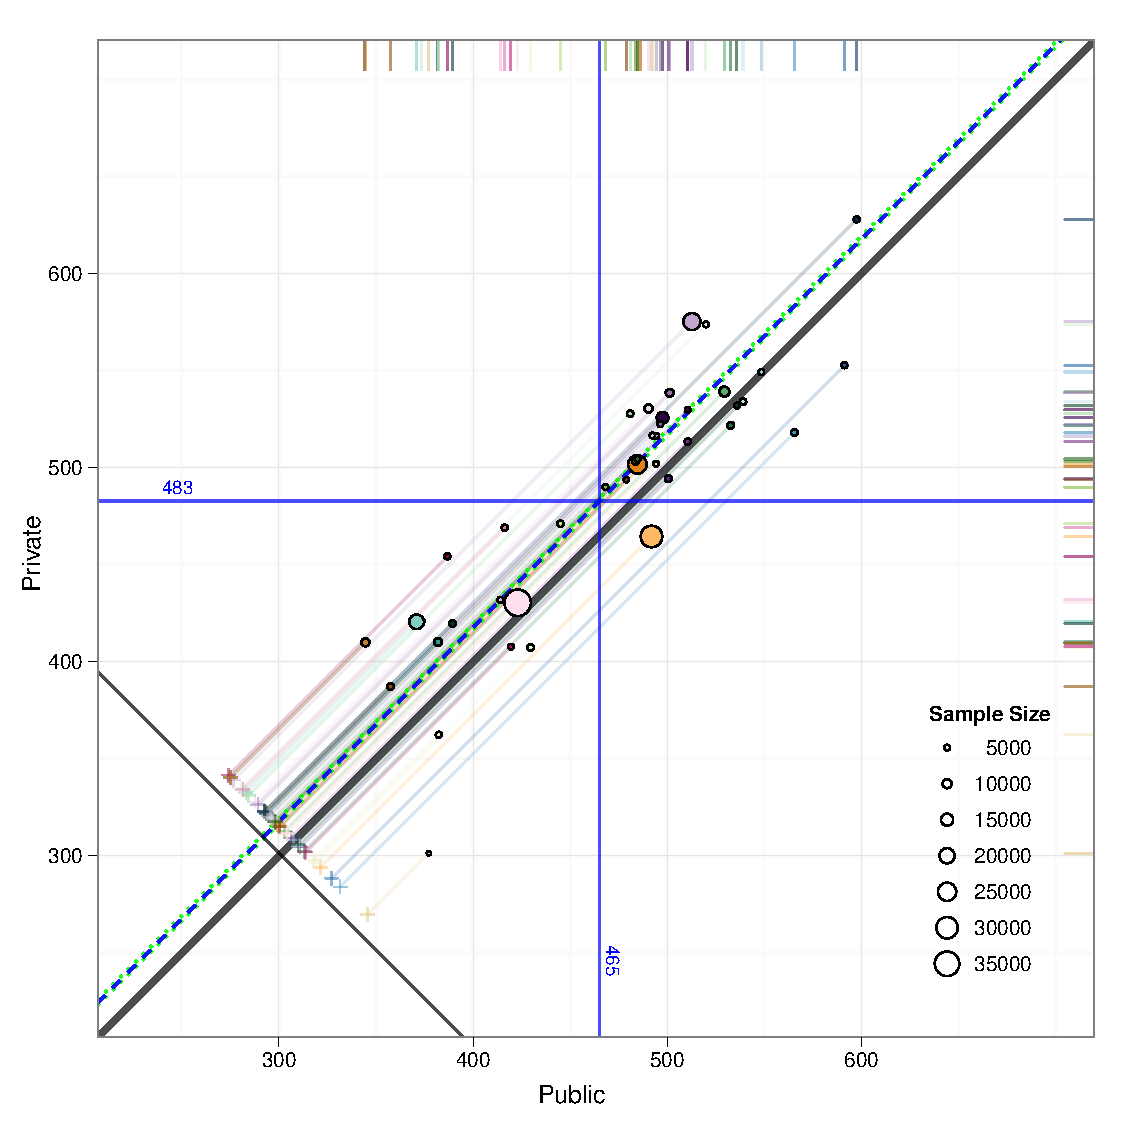
\includegraphics{multilevelPSA-021}
\caption{Multilevel PSA Assessment Plot: Mathematics}
\label{fig:circpsamath}
\end{center}
\end{figure}

\begin{Schunk}
\begin{Sinput}
> p = plotpsa.multilevel.psa(multilevelPSA=results.psa.math, sd=NULL, 
+ level1.points=TRUE, ylab='Country', jitter=FALSE) + 
+ opts(axis.text.y=theme_text(size=8, hjust=1)) + 
+ ylab('Difference Score (private - public)') + opts(legend.position=c(-1,-1))
\end{Sinput}
\end{Schunk}

\clearpage
\begin{figure}[tp]
\begin{center}
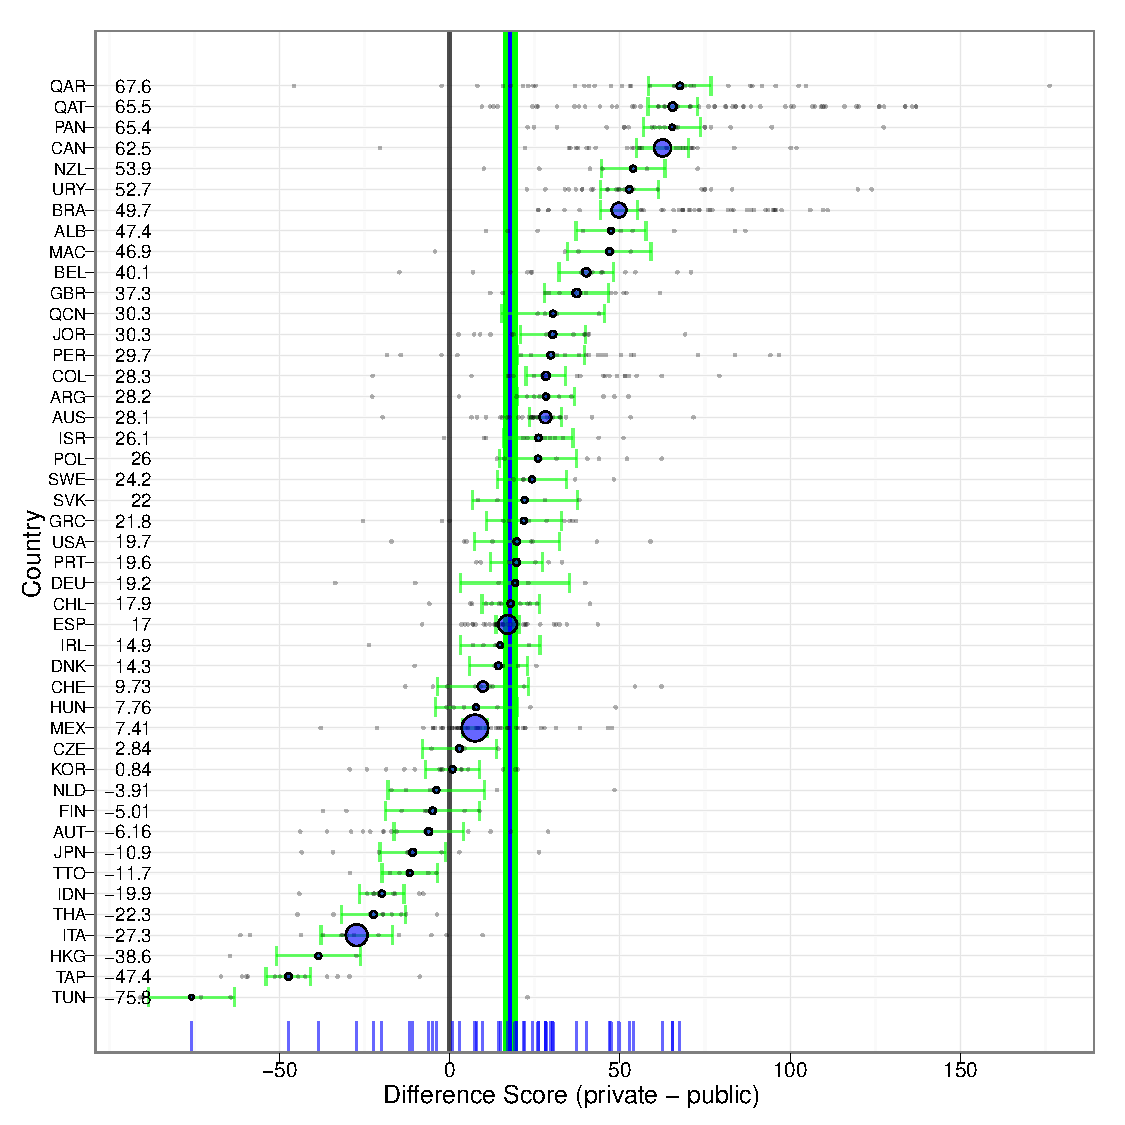
\includegraphics{multilevelPSA-023}
\caption{Multilevel PSA Difference Plot: Mathematics}
\label{fig:diffpsamath}
\end{center}
\end{figure}


\end{document}
